\documentclass[11pt, a4paper]{article}\usepackage[]{graphicx}\usepackage[]{color}
%% maxwidth is the original width if it is less than linewidth
%% otherwise use linewidth (to make sure the graphics do not exceed the margin)
\makeatletter
\def\maxwidth{ %
  \ifdim\Gin@nat@width>\linewidth
    \linewidth
  \else
    \Gin@nat@width
  \fi
}
\makeatother

\definecolor{fgcolor}{rgb}{0.345, 0.345, 0.345}
\newcommand{\hlnum}[1]{\textcolor[rgb]{0.686,0.059,0.569}{#1}}%
\newcommand{\hlstr}[1]{\textcolor[rgb]{0.192,0.494,0.8}{#1}}%
\newcommand{\hlcom}[1]{\textcolor[rgb]{0.678,0.584,0.686}{\textit{#1}}}%
\newcommand{\hlopt}[1]{\textcolor[rgb]{0,0,0}{#1}}%
\newcommand{\hlstd}[1]{\textcolor[rgb]{0.345,0.345,0.345}{#1}}%
\newcommand{\hlkwa}[1]{\textcolor[rgb]{0.161,0.373,0.58}{\textbf{#1}}}%
\newcommand{\hlkwb}[1]{\textcolor[rgb]{0.69,0.353,0.396}{#1}}%
\newcommand{\hlkwc}[1]{\textcolor[rgb]{0.333,0.667,0.333}{#1}}%
\newcommand{\hlkwd}[1]{\textcolor[rgb]{0.737,0.353,0.396}{\textbf{#1}}}%
\let\hlipl\hlkwb

\usepackage{framed}
\makeatletter
\newenvironment{kframe}{%
 \def\at@end@of@kframe{}%
 \ifinner\ifhmode%
  \def\at@end@of@kframe{\end{minipage}}%
  \begin{minipage}{\columnwidth}%
 \fi\fi%
 \def\FrameCommand##1{\hskip\@totalleftmargin \hskip-\fboxsep
 \colorbox{shadecolor}{##1}\hskip-\fboxsep
     % There is no \\@totalrightmargin, so:
     \hskip-\linewidth \hskip-\@totalleftmargin \hskip\columnwidth}%
 \MakeFramed {\advance\hsize-\width
   \@totalleftmargin\z@ \linewidth\hsize
   \@setminipage}}%
 {\par\unskip\endMakeFramed%
 \at@end@of@kframe}
\makeatother

\definecolor{shadecolor}{rgb}{.97, .97, .97}
\definecolor{messagecolor}{rgb}{0, 0, 0}
\definecolor{warningcolor}{rgb}{1, 0, 1}
\definecolor{errorcolor}{rgb}{1, 0, 0}
\newenvironment{knitrout}{}{} % an empty environment to be redefined in TeX

\usepackage{alltt}
\usepackage{graphicx}
\usepackage{lipsum}
\usepackage{verbatim}
\usepackage[vmargin=3cm, hmargin=2cm]{geometry}
\usepackage{url}
\usepackage{hyperref}
\usepackage{fancyhdr}
\usepackage{color}
\usepackage{amsmath, amssymb}
\usepackage{longtable}
\usepackage{lscape}
\usepackage{natbib}
\usepackage{xspace}
\usepackage{textcomp}
\usepackage{float}
\usepackage{booktabs}
% =======================================

% bibliography
\bibliographystyle{apalike}
\IfFileExists{upquote.sty}{\usepackage{upquote}}{}
\begin{document}
\tableofcontents
\bigskip

\section{Intro}
Cells are one of the fundemental units of life. They show a broad complexity and diversity. The identity and function is determined by The identity of a cell is defined by it A human consist of estimated $4*10ˆ13$ cells. 
Single-cell RNA sequencing (scRNA-seq) was first published by \citet{tang2009mrna}. A typical scRNAseq workflow consist of the isolation of single cells, extraction of RNA, cDNA libary preparation, amplification and  sequencing of the libraries (Fig workflow). Many of the steps are similar to bulk RNA-seq pipelines. In comparison to traditional bulk RNA-seq methods its possible to measure transcriptomes from single cells. This allows to adress new biological questions like the identification of rare cell populations, measure the frequency of cell types in tissues, characterizing differences in similar cell-types, investigating the heterogeneity in cell states or cell lineages \citet{andrews2017identifying}. 
Differences between bulk experiments are the lower sequencing depth (100000 - 5 million reads per cell), higher variability and more outliers (Chen et al. 2017).  
scRNA-seq data suffers from technical noise, multiple cells in a library, batch effects and low capture efficiency. 
Batch effects occur when different biological conditions are processed in different batches, making the deconvolution between technical noise and biological effect impossible. Wehnever pssoble this should be avoided by a approbiate experimental design that allows for the statistical deconvolution between unwanted and wanted variation. In scRNAseq the single experimental unit is the cell, making this approach not always possible. Different cells in a experiment may need different sample processing or their biological differences affects the downstream analyses \citep{wagner2016revealing}. 

Doublets occur when multiple cells proccesed in the same library and is mainly a problem for droplet based methods. Starting amounts of the library preparation can be as low as 10 picogramms of total RNA. Two main problems are arising to the low starting amount. The heavy amplification and low capture efficiency.
 Low and moderate expressed genes are not captured during the reverese transcription, which  leads to dropouts of genes and to a zero-inflated gene expression. 
 To deal with technical noise unique molecular identifiers (UMI) counts or spike inns from the External RNA Control Consortium  (ERCC) are used. UMI are short random barcodes attached to the single stranded cDNA in the reverse transcriptase process. By counting the unique UMI reads aligned to the genome an estimated tag count is obtained. ERCC is added prior to amplifaction. Under the assumption that the amplification of the endogenous and exogenous RNA is similar they can be used for library size normalization and to remove technical noise. 

A wide variety of scRNA-seq protocols exists, differing in throughput, full transcript or 3'sequencing, costs and automatization.
Depending on the research question a variety of protocols exist for high throughput or small scale experiments exist. Small-scale protocols are classical PCR plate based methods ( Smartseq2, CELL-seq citation ) or methods in which cell-isolation and library preparation is combined into one protocol (Marsseq). A typical protocol small scale protocol is the plate-based PCR SMARTseq2.  Libraries are full transcript sequenced, using a standart Ilumina sequencing. Typically hundreds of cells are processed and ERCC are used for normalization. Drop-seq is droplet based method using microfluidic cell sorting (e.g. FACS) , allowing for the processing of thousand of cells. Sequencing is 3'end and generally uses UMI. One of the highest throughputs is achieved by 10xChromium, allowing for the sequencing of tens of thousand s of cells. The method is again droplet based, sequencing is 3' end and UMI based. 
Droplet methods like Drop-Seq or 10xChromium are used for high throughput sequencing. Thousand s to Millions of cells can processed, albeit normally with a low sequencing depth.

In general scRNA-seq experiments consist of high-dimensional data. High-dimensional data suffers from the curse of dimensionality (Wagner 2016). Distances in high dimensional data become instable and subpoplutaions cannot be sepereated (Hemberg 2017). Additionaly computational requirements are high. Reduction of the dimension is done by two approaches. Using linear or non-linear for projectiont of the data from the original high-dimensional to a lower-dimensional latent space. Another approach is by feature selection. This is normally done in removing uninformative genes. 




\section{Methods}

\subsection{Clustering Methods}

\subsection{Clustering Methods}

\paragraph{tSNE}
 tSNE (t-distributed stochastic neighborhood embedding) is a non-linear mapping \citet{an2013barnes} for dimensionality reduction. Stochastic neighbor embedding (SNE) transforms euclidean distances to conditional probabilities $p_{j|i}$. That is the probability of \(x_j\) is the nearest neighbor of $x_i$ under a Gaussian centered at $x_i$. The low dimensional counterpart $q_{i|j}$ is similar with a Gaussian centered at $y_i$ and variance $1/sqrt(2)$. SNE minimizes the divergence between $p_{j|i}$ and $q_{j|i}$ using the Kullback-Leiber divergence. 
tSNE implements a Student-t distribution for the low dimensional space and symmetric version of the cost function to simplify optimization and to overcome the crowding problem.
In tSNE the cost function uses joint probabilities $p_{ij}$ and $q_{ij}$  instead of conditional probabilities. 
To deal with large data sets the Barnes-Hut implementation uses random walks on the nearest neighbor network with a PCA step to reduce the dimensionality of the high dimensional data.

\paragraph{K-means}
K-means clustering finds predefined number of centers $k$ and assignments \citep{hartigan1979algorithm} such that their within-group sum of squares is minimized. $k$ cluster centers are randomly assigned.
Each data point is then assigned to the nearest center using Euclidean distances. The centers are then recomputed using the average of the data points that are assigned to each of the $k$ centers. This procedure is iterated until the algorithm converges. The assigning of the centers is random. Also it's not guaranteed to find the global minimum.  As the variable with the largest range can dominate the other others, it is often advised to use scaled data. 



\paragraph{pcaReduce}
pcaReduce uses PCA and kmeans clustering to find the number of clusters in the reduced dimension given by PCA \citep{yau2016pcareduce}. An assumption of pcaReduce is  that large classes of cells are contained in low dimension PC representation and more refined (subsets) of these cells types are contained in higher dimensional PC representations. Given an gene expression matrix, the clustering algorithm starts with a K-means clustering on the PCA projections $Y_{n\times q}$ with $q+1$ clusters. Where $n$ are the cells and $q$ are the number of PC's. The number of initial clusters $k$ is typically around 30,  guaranteering that most cell types are captured. For all pairs of clusters the joint probabilities are computed.  Two cluster are merged together by selecting the pair with the highest probability or by sampling proportionally by the joint probabilities. The number of clusters is now decreased to $K-1$. Next, the PC with the lowest variance is deleted. And a k-means clustering with $K-2$ centers is performed. This process is repeated until only one single cluster remains. Using pcaReduce $q$ cluster partitions with $k-1$ clusters are obtained.

\paragraph{SC3}
Implemented in the SC3 method is a gene and cell filtering and log transformation step of the expression matrix \citep{kiselev2017sc3}. The filtered expression matrix is then used to compute  Euclidean, Pearson and  Spearman dissimilarity measures. By PCA or Laplacian graphs  a lower dimensional representation of the data is obtained.  K-means clustering is then performed on the $d$ different dimensions. Next, a consensus matrix of the different clustering results is computed. The consensus matrix is a binary similarity matrix with 1 if two cells belong to the same cluster and 0 otherwise. The consensus matrix is obtained by averaging the individual clustering(how?). The last step is a hierarchical clustering step with complete linkage. The cluster is inferred by the $k$ level of hierarchy, where $k$ is supplied by the user. To reduce run time SC3 changes the clustering when supplied with more than 5000 cells. Randomly selected cells are then used for the clustering approach described before. These subpopulations are then used to train a Support Vector Machine to infer the remaining cells.

\paragraph{SNNcliq}
SNNcliq  computes a a shared nearest neighbor graph based on the the high-dimensional data. \citep{xu2015identification}. Nodes are the data points and weighted edges are the similarities between the data points. Cells are defined as a cluster if they have a defined number of edges between them, forming a "clique". 
A similarity matrix using Euclidean or other similarity measures is computed. Using this similarity matrix the  k-nearest-neighbors (KNN) for each data point are listed. The parameter KNN has to be supplied by the user. Edges between data points are assigned if they share at least one KNN. The weights of the edges are defined by a function of the number of nearest neighbors and their respective ranks. 
Identification of clusters is done by finding quasi-cliques associated with each node and merging them to unique clusters.
To find maximal quasi-cliques a greedy algorithm is used. A node induces a sub graph  which consists of all its neighbor nodes and edges. For each node a local degree is computed and a node removed from the sub graph if the degree is lower as a threshold which is proportional to the size of the clique. The threshold is supplied by the user and is typically set to 0.7. Next the degrees between the nodes are recomputed and the process is repeated until no more nodes can be removed. A sub graph  is assigned to a quasi clique if it contains more than three nodes. To reduce redundancy quasi-cliques that are completely included in other cliques are removed.
Clusters are then identified by merging the quasi-cliques. For each pair an overlapping rate is computed. If it exceeds a predefined threshold m the sub graphs are merged. Merging in different orders lead to different results so pairs with larger sizes are prioritized.

\paragraph{SIMLR}
Most clustering method rely on standard similarity metrics like euclidean distances \citep{wang2017visualization}. SIMLR uses a weighted function of multiple kernels to compute a distance matrix. Assumptions are that the matrix has a block-diagonal structure , where the blocks represents the clusters $c$. The Kernels are Gaussian kernels with a range of hyper parameters defining the variance of each kernel. The similarities are then used for data visualization with tSNE or clustering using k means and the latent space representations of the similarities.
\paragraph{ZINB-WaVE}
The method is based on a zero-inflated negative binomial (ZINB) model that accounts for the zero inflated, over dispersed nature of scRNAseq count data\citep{risso2017zinb}. 
Based on the preprocessing steps given by the authors genes with less than 5 counts per feature were filtered out. Also it is recommended to use only high variable genes. ZINB-Wave is based on Factor analysis.

\paragraph{dbscan}
dbscan is a density based clustering method. A general assumption is that high density areas are well separated by low-density areas.  The methods work with euclidean distances, as well as other distant measures. Data points are defined as core points, border points and noise points. A core point is defined as point that lies in a neighborhood of a predefined number of other points. Border points are in the neighborhood of core points. Noise points are all other points. 
Each of the points were labeled as core, noise or border points. Edges between all core points that lie inside a neighborhood $\epsilon$ were assigned. Connected core points belong to the same cluster. Border points are then assigned to the cluster of the respective core points. The border points can belong to different clusters so there's no unique solution. The number of cluster is not predefined and the cluster can have different forms, but not densities. A disadvantages is that the method performs badly with high dimensional data. So a dimensional reduction step is recommended.
\paragraph{CIDR}
Clustering through Imputation and Dimensionality Reduction (CIDR) takes the high dropout rate in scRNA seq data into account. CIDR uses TPMs as expression data. The method splits the squared euclidean distance in three terms. One in which both genes $k$ for the pairs $i$ an $j$ are non-zero, one in which one gene is zero and both are zero. The authors state that only the cases were one gene is zero has an strong influence on the distances and the subsequent  dimension reduction and clustering. To reduce the dropout-induced zero inflation, the method imputes the third term by its expected value given the distribution of the dropouts. CIDR works basically in five steps. (i) Find features that are dropout candidates. That is genes that show a expression level below a threshold $T$. (ii) Find the empirical drop-out probability $\hat P(u)$ using the whole data set. (iii) Calculation of dissimilarity using euclidean distances together with pairwise imputation process. Features that fall below the threshold $T$ are imputed using a weighting function. The weighting is based on the probability of being a drop-out. (iv) Dimension reduction using PCA on the imputed distance matrix. (v) Hierarchical clustering using the first few PCs. The number of PC can be determined by several methods. Here we use a implemented variation of the scree method. 
\paragraph{Seurat}
Seurat uses raw counts, filtering is done gene- and cell wise. A user specified threshold for the minimum number of expressed features per cell and minimum number of gene wise expression per cell. Scaling, log transformation and normalization of the counts is done with a scale factor of $10000$, a log2 transformation.... In second gene filtering step low variance genes are filter out. Clustering is finally done using PCA and a smart local moving algorithm (SLM). Here a resolution parameter defines the number of clusters.

\paragraph{ZIFA}
ZIFA is a dimensionality reduction technique for scRNA-seq data. To reduce the dimensionality a probabilistic Principal Components Analysis (PCA) that includes a 
zero inflated model to account for dropout events. 
\paragraph{Linnorm }
The main objective of Linorm is normalization and transformation of count data\citep{yip2017linnorm}. It includes functions for Sub population analysis by t-SNE or PCA Kmeans clustering and hierarchical clustering. Raw counts, CPM , RPKM, FPKM and TPM can be provided. 
Main assumption is a existing homogeneously expressed gene set. Using this gene subset, and by ignoring zero counts,  the normalization and transformation parameters are calculated. After normalization the expression values should show homoscedasticity and normality. First the values are scaled by library size. Low count genes  and genes that show high technical noise are filtered out. By default genes showing a non-zero expression in at least 75 \% or retained. Note that this threshold is set to maintain at least three non-zero cells per gene to calculate the skewness of the gene distributions. Based on the increasing sample size in scRNA-seq data this parameter can be less strict. By gradually increasing this threshold only genes which show  negative correlation between the mean and the standard deviation (SD) is assured. 
A locally weighted scaterrplot smoothing (LOWESS) curve is fitted on mean vs. SD relationship. The SD is scaled and outliers based on the SD are removed. Next genes that show a high skewness are filtered Out as well. The data is then transformed using a modified log transformation.
\paragraph{TSCAN}
TSCAN uses a unsupervised pseudo time algorithm for cell ordering \ref{ji2015tscan}. PCA dimension reduction on the Preprocessed gene expression data is performed. Preprocessing is done by log transformation and adding a pseudo count. Low expressed genes are filtered out based on the zero-proportion and their covariance. Clustering done by model-based clustering. 
The travelling salesman problem (TSP) is then solved by a minim spanning tree. The user can then define the starting/ending point through the available biological information and compute a pseudo time ordering score. 



\subsection{Data Sets}

\paragraph{\citet{kumar2014deconstructing}} 
Kumar et al. used $Dgcr8$-knockout and V6.5 variotypes from mouse embryonic stem cells (mESCs). Cells were cultured on serum plus leukaemia inhibitory factor (LIF) or under Erk and GSK3 signalling inhibition (2Li). The authors investigated the expression of pluripotency factors and their involvement in heterogeneity of pluripotent stem cells. Sequencing was done using a Fluidigm C1 system and following a SMARTer protocol.  The experimental design is confounded, as the conditions and batches are identical.

\paragraph{\citet{trapnell2014dynamics}} 
\citet{trapnell2014dynamics} used human skeletal muscle myoblast cells to investigate temporal differentiation. Cells were expanded under high-mitogen conditions. Differentiation is induced by switching to low-serum medium. Cells were captured before switching to low-serum medium (T0) , after 24 h (T24) and 48h (T48). Between 49 and 77 cells were isolated at each time point and used for single mRNA-Seq library preparation. Libraries were sequenced with paired-end sequencing on a HiSeq 2500 (Illumina) platform. Sequencing depth was ˜4 million reads per library. 
The Authors excluded libraries that contained fewer than 1 million reads. The three different biological batches were sequenced separately and the experiment is possibly confounded.

\paragraph{\citet{koh2016atlas} }
H7 human embryonic stem cells (hESCs) were used to study human mesoderm developement. Starting from undifferentiated H7 hESCs several differentation stages, sorted by time point and further refined by fluorescence activated cell sorting (FACS) were isolated. Finally 9 different cell lines were obtained:  undifferentiated H7 hESCs (H7hESC), anterior primitive streak populations (APS) , mid primitive streak populations (MPS), lateral mesoderm (D2LtM), FACS-purified DLL1+ paraxial mesoderm populations (DLL1pPXM), early somite progenitor populations (ESMT) , PDGFRα+ sclerotome populations (Sclrtm) and D2.25Smtmrs and dermomyotome populations(D5CntrlDRmmtm).
Before library preparation, cells were checked for degradation and if the Fluidigim reaction chambers contained multiple cells. In total 10 different cell types were then sequenced on a Fluidigm C1 system and following  SMARTer protocol. Sequencing depth was 1 to 2 million reads per cell. 
Note that the authors discarded libraries with less than one million reads during the quality control process, finally using 498 out of 651 cells.

\paragraph{ \citet{zheng2017massively}}
FACS-purified fresh periphelar blood mononuclear cells (PBMCS) sub-populations were sequenced using a droplet-based system. Gene filtering was done using only genes that showed at least one UMI count in at least one cell. FACS purity was 98 - 99 percent. Four of these purified filterd cell populations; namely CD19+ B, CD8+CD45RA+ naive cytotoxic, CD14+ monocytes and CD4+/CD25+ regulatory t cells were selected and used for the clustering analyses. CD19+ B and  CD14+ monocytes cells are distinct cell populations. Whereas CD8+CD45RA+ naive cytotoxic cells and  CD4+/CD25+ regulatory t cells are not distinguishable by tSNE dimension reduction and kmeans clustering.
To construct an artificial population 200 cells each were subsampled from these libraries and merged to obtain a single expression matrix.

\paragraph{Simulated dataset }
Using the Splatter package \citep{oshlack2017splatter} expression data were simulated. Parameters for the simulation were estimated from a subpopultaion of the Kumar dataset.  Embryonic stem cell variotypes V6.5 with signalling inhibition and LIF  were used for the estimation.  Four subpopulation with  37,72 ,  253 and 134 cells were simulated. The probabilies that a gene is differentially expressed per group were 0.05,0.1,0.2 and 0.4. 


\subsection{Transformation}


\begin{figure}[!h]
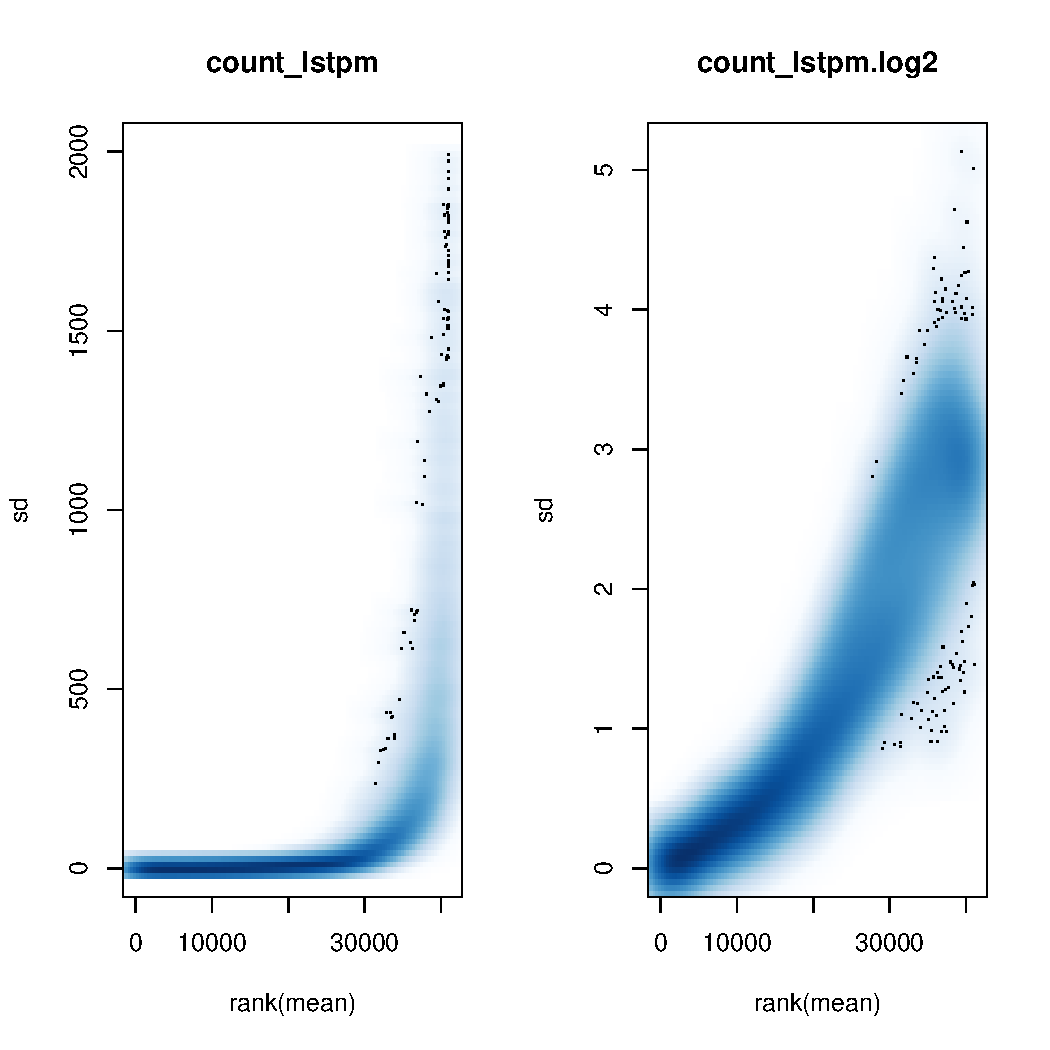
\includegraphics[width=5 in]{/Users/angeloduo/Desktop/masterarbeit/scRNAseq_clustering_comparison/results/QC_data/meanvarplots_trapnell2014.pdf}
\caption{transformations Trapnell 2014.}
\label{fig:transtrapnell}
\end{figure}

\begin{figure}[!h]
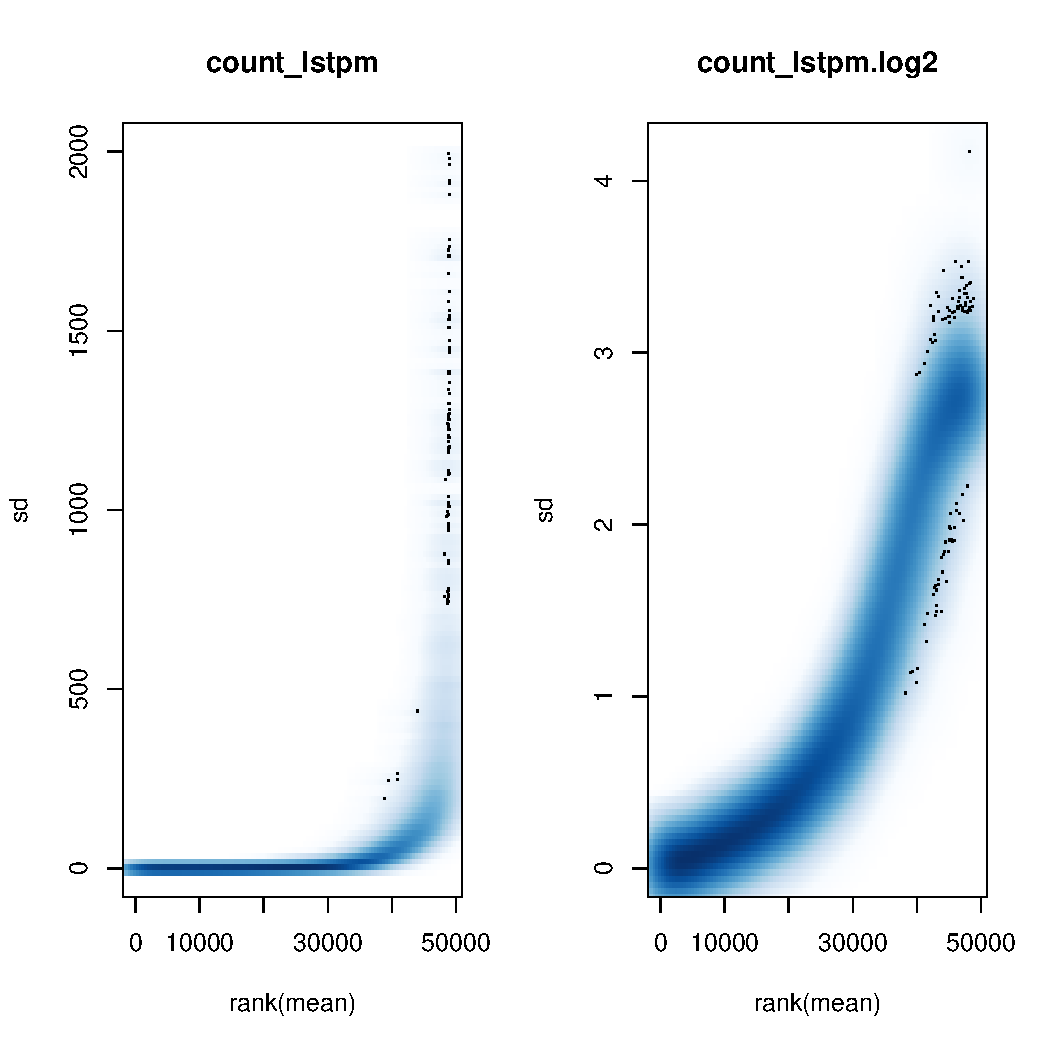
\includegraphics[width=5 in]{/Users/angeloduo/Desktop/masterarbeit/scRNAseq_clustering_comparison/results/QC_data/meanvarplots_koh2016.pdf}
\caption{transformations Koh2016.}
\label{fig:transkoh}
\end{figure}

\begin{figure}[!h]
\includegraphics[width=5 in]{/Users/angeloduo/Desktop/masterarbeit/scRNAseq_clustering_comparison/results/QC_data/meanvarplots_zhengmix2016.pdf}
\caption{transformations Zheng 2016.}
\label{fig:transzheng}
\end{figure}

\begin{figure}[!h]
\includegraphics[width=5 in]{/Users/angeloduo/Desktop/masterarbeit/scRNAseq_clustering_comparison/results/QC_data/meanvarplots_simDataKumar.pdf}
\caption{transformations simDataKumar.}
\label{fig:transsim}
\end{figure}

RNA-seq data may suffer from heteroscedasticity, skewness and a mean-variance dependency \citep{zwiener2014transforming}. Genes with higher mean have on average a higher variance across cells leading to unequal variances between different genes. 
To handle this properties different transformation were considered. A Logarithmic transformation with base 2, arcus sin transformations and  a variance-stabilizing transformation (VST)\citep{huber2002variance} from the DESeq package. Log transformations will have an impact on extreme values and after transformation the distribution should be more normally distributed. However, log transformations do not address the problem of heteroscedasticity. Arcus sin transformation should deal with extreme values and equalize the variances. After transformation the mean and the variances should be independent. VST address the problem of extreme values and unequal variances across genes. After such transformation, the mean and the variances of the genes should be independent. Box-Cox transformations address the problem of extreme values and the data should be less skewed. Using log transformation and VST the mean-variance dependence is less extreme ( see Figure ). Still, for means in the lower-mid range, the variances are not equal. 

\subsection{Filtering and normalization}

\begin{figure}[!h]
\includegraphics[width=4 in]{/Users/angeloduo/Desktop/masterarbeit/scRNAseq_clustering_comparison/results/QC_data/hist_Kumar2014.pdf}
\caption{Histogram of Kumar 2014.}
\label{fig:histkumar}
\end{figure}

\begin{figure}[!h]
\includegraphics[width=5 in]{/Users/angeloduo/Desktop/masterarbeit/scRNAseq_clustering_comparison/results/QC_data/hist_Trapnell2014.pdf}
\caption{Histogram of Trapnell 2014. }
\label{fig:histtrap}
\end{figure}

\begin{figure}[!h]
\includegraphics[width=5 in]{/Users/angeloduo/Desktop/masterarbeit/scRNAseq_clustering_comparison/results/QC_data/hist_Koh2016.pdf}
\caption{Histogram of Koh 2016. }
\label{fig:histkoh}
\end{figure}


\begin{figure}[!h]
\includegraphics[width=5 in]{/Users/angeloduo/Desktop/masterarbeit/scRNAseq_clustering_comparison/results/QC_data/hist_simDataKumar.pdf}
\caption{Histogram of simDataKumar. }
\label{fig:histsim}
\end{figure}



\begin{figure}[!h]
\includegraphics[width=5 in]{/Users/angeloduo/Desktop/masterarbeit/scRNAseq_clustering_comparison/results/QC_data/comparison_panel.png}
\caption{Comparison between the data sets. Based on compare function of Splatter.}
\label{fig:compare}
\end{figure}

The quality control of the data sets follows \citep{lun2016step}.
Length scaled and count scaled transcript per million were used for the data sets Kumar, Trapnell and Koh. The Zheng dataset contains UMI counts. First, genes that are not expressed in any cell are removed to reduce the size of the expression matrix.
To find potential outliers PCA on the phenotype characteristic (example) of each cell can be used (Figure \ref{fig:qckumar}, \ref{fig:qctrapnell}, \ref{fig:qckoh}, \ref{fig:qczheng}; a ). The Kumar, Trapnell and Zheng data show some potential Outliers cells. 
Cells with log10-library sizes that are more than 3 median absolute deviations (MADs) below the median log-library size were filtered out (Figure \ref{fig:histkumar}, \ref{fig:histtrap}, \ref{fig:histkoh}, \ref{fig:histsim}). The same filtered was used with respect to the total number of genes per cell.  For the Kumar and the Zheng dataset ERCCs and MT counts were available. Cells with large proportions of ERCC or mitochondrial RNA are seen as low quality cells. In the Kumar dataset cells with a ERCC proportion above 3 MADs are as well removed. The same filter was used for mitochondrial gene expression in the Zheng data.
For the Trapnell 2014 data set information about the cell quality was available. In this dataset cells that were marked as debris or if a single library consist of more than one cell were as well filtered out. Leaving 531 cells in the Koh dataset, 246 in the Kumar dataset and 222 in the Trapnell dataset. The filtering was less strict in the Koh data set compared to the original analysis 2016 were they retained 498 cells. 
Low-abundance genes influence the mean- variance trend. Here low-abundance genes are filtered by their average counts Figure \ref{fig:qckumar}, \ref{fig:qctrapnell}, \ref{fig:qckoh}, \ref{fig:qczheng}; d ). For the Kumar , Trapnell , simDataKumar and Zheng data genes with average counts less than one are removed. The Zheng data set had a shallower sequencing depth. features which are not expressed in at least two cells are removed.
By fitting a linear model on the PC scores against the total number of features 
To find batch effects a linear model regressing the PC values against the total features was used\citet{lun2016step}. Whereas for Kumar and Koh PC1 has a high correlation with the number of features.

Another examination of the technical factors that have  an influence on the variances can Be done using the marginal variances. For that a linear model with the expression values per gene as response variables and a chosen  explanatory variable is fitted. The correlation coefficient can than be seen as the marginal explained variance for the explanatory variables.
In  Kumar similar amount  of the variance is explained by the total number of genes, the proportion of ERCC and the phenotype. This indicates that the data set is heavily influenced by batch effects. They same holds in the Trapnell data, but on a lower scale. Variance in Koh data is largely influenced by the phenotype and to a lesser extend by total number of genes and the top 200 features. 
Zheng is largely dominated by the biological variation with the other explanatory factors contribution only marginally to the complete variances.


scRNA-seq data has an excess of zero counts. These can be split into systematic, semi-systematic and stochastic zeros (Lun, 2016). Systematic zeros are silent across all cells. These features were removed prior to the analysis. Stochastic zeros are zero counts that were obtained due to sampling. It affects genes with a count distribution near zero. Semi-systematic zeros come from genes that are silent in a sub population of cells. Different methods exist to normalize RNA-seq data like TMM normalization, DEseq normalization and by library size. However, none of these methods are designed to deal specifically with the zero-inflated nature of scRNA-seq data.
Another approach is the normalization by spike-inn. This approach is not feasible as no or only a limited number of spike-inn counts were present.  Here normalization through pooled cells was used \citet{lun2016pooling}. Counts from different cells were pooled together. The summed count size was then used to estimate size factor. The size factors for the pooled cells were then  "deconvoluted" into cell-based factors (Lun et al., 2016). By default the expression values are log transformed.


\begin{figure}[!h]
\includegraphics[width=5 in]{/Users/angeloduo/Desktop/masterarbeit/scRNAseq_clustering_comparison/results/QC_data/qc_summary_kumar.png}
\caption{QC summary of Kumar 2015. }
\label{fig:qckumar}
\end{figure}

\begin{figure}[!h]
\includegraphics[width=5 in]{/Users/angeloduo/Desktop/masterarbeit/scRNAseq_clustering_comparison/results/QC_data/qc_summary_trapnell.png}
\caption{QC summary of Trapnell 2014. }
\label{fig:qctrapnell}
\end{figure}

\begin{figure}[!h]
\includegraphics[width=5 in]{/Users/angeloduo/Desktop/masterarbeit/scRNAseq_clustering_comparison/results/QC_data/qc_summary_koh.png}
\caption{QC summary of Koh 2016. }
\label{fig:qckoh}
\end{figure}

\begin{figure}[!h]
\includegraphics[width=5 in]{/Users/angeloduo/Desktop/masterarbeit/scRNAseq_clustering_comparison/results/QC_data/qc_summary_zheng2016.png}
\caption{QC summary of Zheng 2016. }
\label{fig:qczheng}
\end{figure}

\begin{figure}[!h]
\includegraphics[width=5 in]{/Users/angeloduo/Desktop/masterarbeit/scRNAseq_clustering_comparison/results/QC_data/qc_summary_simDataKumar.png}
\caption{QC summary of simDataKumar. }
\label{fig:simDataKumar}
\end{figure}

\begin{figure}[!h]
\includegraphics[width=5 in]{/Users/angeloduo/Desktop/masterarbeit/scRNAseq_clustering_comparison/results/QC_data/qc_summary_simDataKumar2.png}
\caption{QC summary of simDataKumar2. }
\label{fig:simDataKumar}
\end{figure}


\subsection{Optimal number of clusters}
Methods to determine the optimal number of clusters are subjective methods as elbow or silhouette plots. In the Elbow plots, the within-cluster sum of square is plotted against a range of clusters. The silhouette plot is a standardized measure of distances between each point inside and outside of the respective cluster. Less subjective is the gap statistic. Here the log within sum of squares is compared to its expectation. The null distribution is expected to be uniformly distributed, it is not clear if this is correct for high dimensional data \citep{tibshirani2001estimating}. Other possible methods are the calinsky criterion, hierarchical clustering....
Here the optimal number of clusters is determined by Elbow plots, clustering is based on kmeans clustering and the within-cluster sum of square thereof.
The elbow plots suggest three clusters for the Kumar dataset, 2 - 5 in the Trapnell data, 3 in in the Zhengmix data (see Figure \ref{fig:transkumar} ). The optimal number of clusters is unclear for the Koh data set. 
Minimization of within sum of squares was also done in the tSNE latent space with 30 dimensions. Here the optimal number of clusters are 3,3, 4 and 6 to 8  in the Kumar, Trapnell, Zheng and the Koh data sets, respectively.

\begin{figure}[!h]
\includegraphics[width=5 in]{/Users/angeloduo/Desktop/masterarbeit/scRNAseq_clustering_comparison/results/plots/optimalk_wss_tsnekmeans.pdf}
\caption{Optimal number of clusters by minimizing within sum of squares based on the latent space of tSNE (30 dimensions) }
\label{fig:wsstsne}
\end{figure}

\begin{figure}[!h]
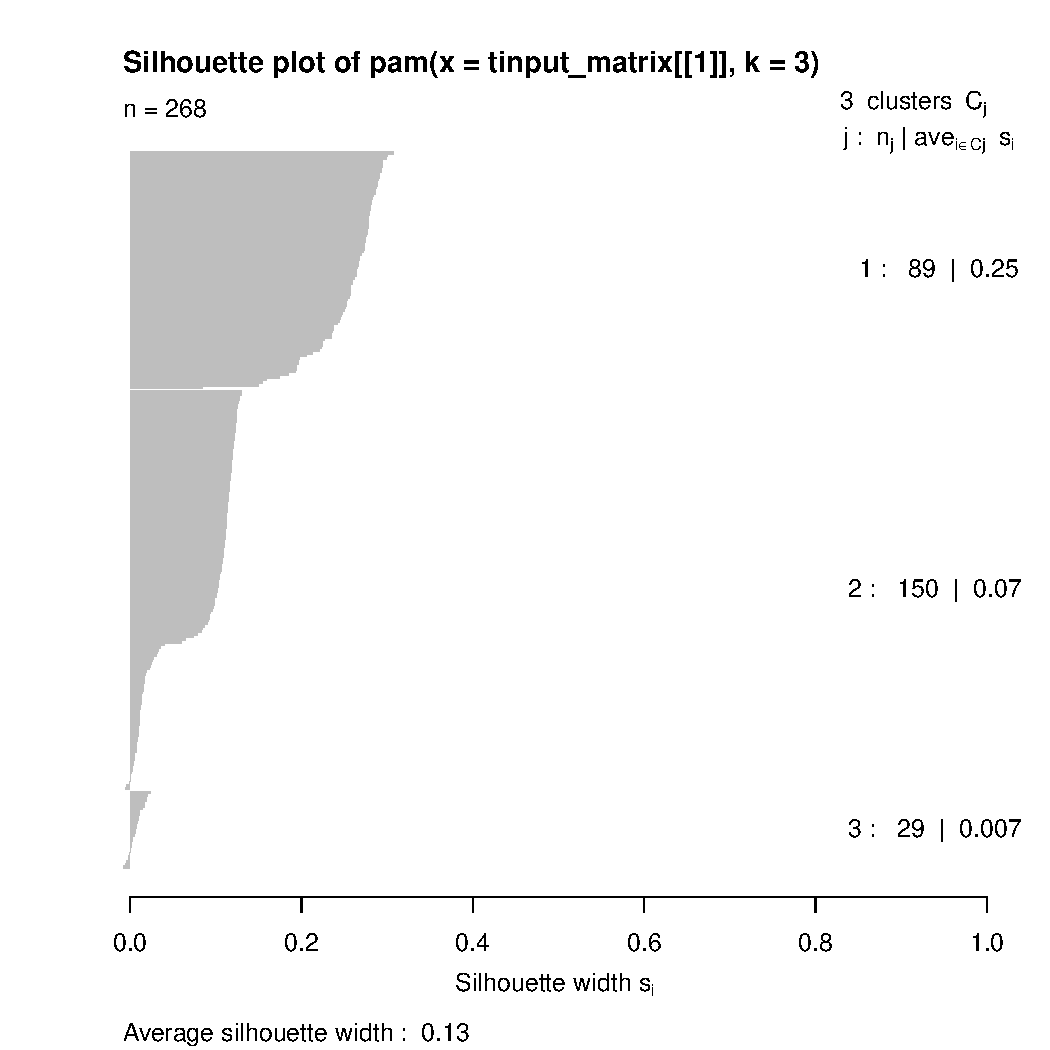
\includegraphics[width=5 in]{/Users/angeloduo/Desktop/masterarbeit/scRNAseq_clustering_comparison/results/plots/optimalk_wss.pdf}
\caption{Optimal number of clusters by within sum of squares based on the full dimensions }
\label{fig:wssorg}
\end{figure}

\newpage
\section{Method}

\begin{center}
\begin{table}[!h]
\footnotesize
\begin{tabular}{ | p{ 2 cm} |  p{ 5 cm}  | p{ 2 cm} | p{ 2 cm} | p{ 0.5 cm} | p{ 0.6 cm} | p{ 0.6 cm} |}
    \hline
    Method & Description & dimension reduction & clustering & zero inflation & normalization & unsupervised \\ \hline
    \hline
     tSNEkmeans & tSNE dimension reduction and kmeans clustering & tSNE & kmeans & no & no & no \\ \hline
    pcaReduce &PCA dimension reduction and kmeans clustering through an iterative process. Step wise merging of cluster by joint probabilities and reducing the number of dimension by PC with lowest variance & PCA & kmeans, hierarchical clustering & no & no &  \\ \hline
     SC3 & PCA  dimension reduction or Laplacian graph. Kmeans clustering on different dimensions. Hierarchical clustering on consensus matrix obtained by kmeans. & PCA & repeated kmeans, hierarchical clustering on similarity matrix of kmeans results & no & no & yes \\ \hline
    SNN-cliq & Shared nearest neighbor  graph based on similarities. Clustering through forming of cliques and subsequent merging. & graph based & merging of cliques & no & no &  \\ \hline
        dbscan & Density based clustering & none &density based clustering & no & no & yes \\ \hline
     SIMLR &  & tSNE & kmeans & yes & no & yes \\ \hline
    CIDR & PCA dimension reduction based on zero imputed similarities. Hierarchical clustering on a number of PC determined by variation of scree method. & PCA on imputed distances & hierarchical clustering& yes & no & yes \\ \hline
   Seurat v1.4 & Nearest neighbor graph based on PCA latent space & HVG and PCA & & no & yes & yes \\ \hline


    \end{tabular}
    \end{table}
\end{center}


\subsection{Evaluation}
Different settings were used for evaluation, under default mode, with filtered and unfiltered data sets. 
In the  simple case the methods were run under the default mode. The run parameters were given either by the default setting of the functions or by examples in the different package vignettes. If the method was able to detect the number of sub populations, the auto detection s was used to infer the number of cluster. In semi supervised methods where the number of clusters had to be provided, the number of cluster given by the cell annotation provided by the authors were used. Depending on the required inputs counts , log transformed counts  or normalized counts  from the  filtered data sets were used. Any filtering steps done by the methods were excluded in this analysis.
For the evaluation with filtered data sets filtering steps were excluded. As in the previous evaluation the inputs were counts, log transformed counts and normalized counts. 
Evaluation with non filtered data sets was done as described before, except that the filtering steps are now included in the methods.
An overview of the different method settings is given by table ...
In a further analysis the clustering methods were tested for different values for the number of clusters $k$. Seurat and dbscan do not allow the setting of the number of cluster. Hence, the number of KNN in Seurat and the size of the neighborhood $\epsilon$ in dbscan was selected.
\subsection{Evaluation metrics}
One evaluation criteria was the Hubert - Arabje Adjusted Rand Index (ARI) for comparing two partitions. The measure is adjusted for chance and 0 if there's no agreement between pairs and 1 if there is full agreement between pairs. The other criteria is the F1 score. It is the weighted average mean between precision and recall. With weights defined by the inverse of the precision and recall. F1 scores can take on values between 0 and 1.The predicted clusters and the "ground truth" were match by the Hungarian algorithm. Some of the clustering methods are unsupervised and the partitions does not need to have the same sizes (non-bipartite). This causes problems with Hungarian algorithm. As a solution the assignment matrix is augmented with dummy columns with the maximum matrix value as its entries.

\subsection{Parameter settings}
For most of the methods the number of cluster is the most important parameter. Other important settings were the kNN, the number of latent space dimensions used for the clustering algorithms or the settings of the filtering and normalization steps.
Here different parameter settings were used to find the optimal settings for each method. First, the methods were run under default mode. Many users will likely run the methods without any fine tuning of the parameters and it was seen important to provide results under this setting. Note that only the methods PCAreduce, SC3, Linnorm, RACEID, TSCAN are completely unsupervised and no parameters have to be provided. For SEURAT and dbscan the number PCs or the number off the kNN have to be defined. CIDR,  RtSNEkmeans, SIMLR need the specification of the number of clusters $k$. For these three methods the parameters setting is equal to the settings described in the next section.
Although its possible to run the methods unsupervised, for many of the methods a fine tuning of the parameters is highly recommended.
Next, methods were run with a the set ground truth of numbers of sub populations. For many of the methods $k$ is a input parameter. However, the methods dbscan and SEURAT allow the setting of $k$ only indirect trough kNN or a resolution parameter. 
To evaluate the methods for the best possible partitions of cells , given the ground truth and evaluated by the use of the ARI score the methods were run under a range of parameters. Whenever possible, the range was chosen such that a clear maximum for the ARI score could be found. A full listing of the parameter settings for each method and run mode is provided in table \ldots .
Next, a brief overview for the chosen parameter setting and the rationale behind it is given.
\paragraph{RtSNEkmeans}
To reduce run time the Barnes-Hut tSNE implementation is used. Perplexity was set to 30 for all data sets. We note that the value of the perplexity can give different tSNE representations, however here the default setting was chosen. tSNE is performed on the first 30 dimensions in the in the PCA latent space .

\paragraph{pcaReduce}
For PCAreduce the range of clusters cannot be specified, instead the number of dimension $q$ in the PCA latent space are to be specified. The results are $q-1$ different clustering solutions, with $k-2$ clusters. For all data sets 30 dimensions were chosen and evaluation was based on the respective number of clusters in the subsequent analysis. The method is based on kmeans clustering and has to be run several times for stable results. Here 50 samples were chosen. Merging of clusters was done by the default sampling proportional to the joint probabilities. 
\paragraph{SC3}
A gene filtering step is implemented in the method.  Filtering steps were included when run with the unfiltered data sets, otherwise the filtering step is excluded. Based on the dropout distribution genes below and above the 10th and 90th percentile  are filtered out before clustering. This seems reasonable for the Kumar, simDataKumar and Koh data sets. However, for the Koh and Zhengmix data set the upper threshold is set to the 99th percentile.
SC3 can run under semi- or unsupervised mode. For the default mode a range of cluster is given, and the number of sub populations is automatically inferred by the method. Otherwise the number of annotated number of sub population is provided. 
\paragraph{SNNCliq}
The connectivity of the quasi-cliques was set to the default value 0.7. Like wise the merging threshold parameter was set to the default of 0.5. The method was run with normalized, filtered data and the number of clusters was set to a range from 3 to 10 in all data sets. SNNclique works on different distance metrics, here the default euclidean distances are used.
\paragraph{SIMLR}
The tuning parameter $k$ was set to the default value of 10 on all runs. The parameter number of clusters $c$ is set accordingly to the run mode.
\paragraph{Seurat}
Implemented in the method are normalization and a gene filtering steps. Filtering criteria are the minimal number of gene expression in the cells and the number of total features per cell. The default setting is zero for both parameters, removing the filtering step. This setting is also chosen when the method is run on the filtered data sets. For the unfiltered data genes which are expressed in less than 5 cells in the Kumar , Trapnell, Koh and simDataKumar were filtered out. For the Zhengmix data the threshold is set to one, according to the filtering used in the QC and normalization steps.
The default log normalization is used, currently the only option. Scale factor for cell-level normalization was set to 10000. As a default no explanatory variables were chosen to be regressed out. The experimental batch would be a natural choice as a covariate, but as the sub populations and the batches are identical for the Kumar and Trapnell data it was chosen not include it. 
The clustering parameters to be defined were a resolution parameter and the number of PCs for the clustering. The resolution parameter was set to the default value of 0.8 . The number of PC was determined by the methods recommended by the authors. Using scree plots and a jackknife permutation test (more exact) to determine the number of principal components. 9, 12, 10 and 15 principal components were used for the Kumar, Trapnell, Zheng and Koh dataset, respectively.
10 percent of cells were used for the number of neighbors in the k-nearest neighbor algorithm. A range of kNN fractions was used to find the the optimal value for the kNN parameter.  A range from 0.5 \% to 40 \% of the total number of cells is used to infer the optimal number for the kNN parameter.
\paragraph{dbscan}
To choose appropriate parameters for the size of neighborhood epsilon and the minimum number of points in neighborhood the k-nearest neighbor distance is used. As a initial number of neighbors 10 percent of cells is used. then for each point the k-NN distance is computed and plot by increasing order. The chosen values for the distances are 280, 410, 35 and 380 for the Kumar, Trapnell, Zheng and Koh data sets, respectively.
The default value for the minimum number of points is 5.
For each of the dataset a range of epsilon around the theoretical optimum was chosen to optimize the clustering results.
\paragraph{CIDR}
CIDR uses three parameter settings; the number of clusters, the number of PCs (nPCs) and the method for hierarchical clustering. By default Ward distances are used in the hierarchical clustering. CIDR is able to infer the number of from 2 to $n$ clusters. By default $n$ is set to $nPC*2+2$. When not run in the default mode we choose the nPC according to a variation of the scree-plot and set the number of cluster accordingly to the respective data set. The number of used PCs for the data sets Kumar, Trapnell, Koh , Zhengmix and simDataKumar are  5, 10, 8, 8 and 3 , respectively.
\paragraph{TSCAN}
The expression matrix is by the default log2 + 1 transformed. In all settings this transformation is used. 
Next, in a filtering step a gene wise threshold for the minimum expression value and a lower bound for the minimum retained fraction of genes that show expression greater than the threshold. As default the minimum expression is set 1 for the transformed counts,  and the minimum fraction is 0.5. The minimum fraction had is set to 0.1 for Zhengmix due to the low sequencing depth of this dataset. For all run methods PCA is performed by default. By default the method infers clusters from a range of 2 to 9 clusters. If run semi supervised the respective number of clusters is given. By default "ellipsoidal, varying volume, shape, and orientation" is used for the model.
\paragraph{Linnorm}
The filtering thresholds are set to the default in all runs, except the Zhengmix data.  For this data set the minimum non-zero expression is to a proportion of 0.1. In the default unsupervised mode the tSNE clustering is performed with $k$ from 2 to 20. In the other runs the respective $k$ per dataset is supplied.




% latex table generated in R 3.4.2 by xtable 1.8-2 package
% Fri Dec 29 11:59:47 2017
\begin{table}[ht]
\centering
\begin{tabular}{rlllll}
  \hline
 & cellfiltering & genefiltering & normalization & autodetect & expressionvalues \\ 
  \hline
tSNEkmeans & no & no & no & no & normcounts \\ 
  pcaReduce & no & no & no & no & normcounts \\ 
  SC3 & no & (yes) & no & yes & normcounts \\ 
  SNNCliq & no & no & no & no & normcounts \\ 
  dbscan & no & no & no & no & normcounts \\ 
  SIMLR & no & no & (yes) & no & normcounts \\ 
  CIDR & no & no & no & yes & normcounts \\ 
  Seurat & (yes) & yes & yes & no & counts \\ 
  TSCAN & no & yes & yes & no & counts \\ 
  ZINBWaVEkmeans & no & no & yes & no & counts \\ 
  RACEID & yes & yes & yes & yes & counts \\ 
  Linnorm & no & (yes) & yes & no & counts \\ 
   \hline
\end{tabular}
\caption{Overview of filtering and normalization steps by method} 
\end{table}


\clearpage

\section{Results}
\paragraph{Clustering}
The annotated number of clusters in the  Kumar, Trapnell and Koh data sets are 3, 3 and 10, respectively. 
In this data sets the true cell population is  given by the authors annotation and it was  chosen as the ground truth. For the simulated data set simDataKumar the number of sub populations are set to 4. The Zheng dataset contained 4 merged cell sub populations. 
For comparison the within sum of squares (WSS) on a range of kmeans clustering was computed.  Similar results were obtained, with exception of the Koh data where the elbow plots suggest 8 clusters.   

For the  methods cidr, pcaReduce, tSNE and kmeans, SC3 , TSCAN , linnorm and SIMLR a range of number of clusters were used. For Seurat a range in k-NN and for dbscan different neighborhood sizes were picked. The Adjusted Rand Index (ARI) is used as a evaluation metric, with the ground truth set by the cell annotation or the given ground truth.

In the Kumar dataset most of the methods show a clear maximum ARI score with three clusters. An exception is pcaReduce where either 3 and 4 clusters achieved a high score. SC3 has it’s maximum with 3 clusters, but higher numbers of clusters reach as well relatively high scores (see Figure \ref{fig:arirangeall}; a). (In SNNClique almost half of all the clustering labels are in disagreement with the annotated cell labeling.)
CIDR, pcaReduce, tSNEkmeans show a maximum score with three clusters in the Trapnell dataset. Whereas for SIMLR and SC3 the optimal number of clusters is 4 and 2 , respectively . 
In the Zheng data CIDR, Linnorm, pcaReduce,  simlr, tSNEkmeans and SC3 had a maximum score value with 4 clusters.  SC3 reached  similar high values for 4 to 7 clusters. In the Koh data pcaReduce, RtSNEkmeans, SC3, SIMLR, cidr and tscan have their maximum at 10, 12, 11 , 8 , 8 and 10 , respectively. Note that the the maximum is not so clear. Except for CIDR, which had a low overall score, all methods have high values on 8 to 12 clusters. In the simulated data set only CIDR and SIMLR had its maximum with 4 clusters, whereas Linnorm, pcaReduce, RtSNEkmeans and TSCAN have a maximum at 3. 



\paragraph{Clustering with the annotated number of cluster, under default mode and with unfiltered data sets}
All methods were run with the number of cluster set to the annotation given by the authors or by the set ground truth. For graph based methods were the neighborhood size had to be define 10 percent of the total cells were used as the  neighborhood size. Others parameters like the number of PC's in Seurat etc. were chosen according to recommendations given by the method manual. For this clustering the filtered dataset was used. 
The partitioning of the clusters were then evaluated using the ARI. Figure \ref{fig:arifilt} shows the Linnorm and pcaReduce performed bad in the simple Kumar dataset.   (why…) No high scores were achieved  in the relatively difficult Trapnell data, with SC3  , RtSNE and Linnorm as the best performing methods. Overall, pcaReduce had the lowest and  SC3  the highest ARI scores  in the filtered data sets. When run under the default method the methods performed similarly. An exception is Linnorm which has higher scores in the Koh, Kumar and simulated data set.
Figure \ref{fig:aridiff1} shows the differences in the ARI scores between the filtered and unfiltered data sets. Here Seurat,  SIMLR and TSCAN perform better in the Koh data. Better scores were also achieved in the Trapnell data by SIMLR, RtSNEkmeans Linnorm and CIDR. Surprisingly RtSNEkmeans had lower scores in the simulated data. As well as pcaReduce in the Kumar and Zhengmix and Linnorm in the Koh, Kumar and simulated data. 
SC3, Seurat, SIMLR, SIMLRlargescale, CIDR and TSCAN performed best with the filtered data sets. Linnorm, pcaReduce, raceID in the filtered dataset. RtSNEkmeans performed similarly under default settings and in the unfiltered data sets.


F1 scores for the Kumar dataset are shown in Figure \ref{}. Most methods are able to assign the correct partitions the three sub populations. However, Linnorm only detected two clusters. pcaReduce is able to correctly partition cluster number three but fails in the sub populations two and three. In the Trapnell data cell population 1 had the highest score. For population 2 and 3 the scores were lower for all methods.
Koh had the highest number cluster, here nine cluster were annotated by the authors. The majority of the methods failed to assign cells to sub population 6 (which is that and why).


\clearpage
\begin{figure}[!h]
\includegraphics[width=5 in]{/Users/angeloduo/Desktop/masterarbeit/scRNAseq_clustering_comparison/results/plots/plot_ari_unfiltered.pdf}
\caption{ARI scores with unfiltered data sets. The number of clusters is determined by the authors annotation. }
\label{fig:ariunfilt}
\end{figure}
\begin{figure}[!h]
\includegraphics[width=5 in]{/Users/angeloduo/Desktop/masterarbeit/scRNAseq_clustering_comparison/results/plots/plot_ari_default.pdf}
\caption{ARI scores with default setting. }
\label{fig:aridef}
\end{figure}

\begin{figure}[!h]
\includegraphics[width=5 in]{/Users/angeloduo/Desktop/masterarbeit/scRNAseq_clustering_comparison/results/plots/plot_ari_filtered.pdf}
\caption{ARI scores with filtered data sets.  The number of clusters is determined by the authors annotation. }
\label{fig:arifilt}
\end{figure}



\begin{figure}[!h]
\includegraphics[width=5 in]{/Users/angeloduo/Desktop/masterarbeit/scRNAseq_clustering_comparison/results/plots/plot_ari_optimalk.pdf}
\caption{ARI scores with filtered data sets. A optimal k is chosen such that the ARI score is maximized. }
\label{fig:arifilt}
\end{figure}

\begin{figure}[!h]
\includegraphics[width=5 in]{/Users/angeloduo/Desktop/masterarbeit/scRNAseq_clustering_comparison/results/plots/plot_ari_smooth.pdf}
\caption{ARI scores with smoothed data sets.  }
\label{fig:arifilt}
\end{figure}


\begin{figure}[!h]
\includegraphics[width=5 in]{/Users/angeloduo/Desktop/masterarbeit/scRNAseq_clustering_comparison/results/plots/plot_ari_rank_all.pdf}
\caption{Ranks of ARI scores.  }
\label{fig:arirank}
\end{figure}

\begin{figure}[!h]
\includegraphics[width=5 in]{/Users/angeloduo/Desktop/masterarbeit/scRNAseq_clustering_comparison/results/plots/plot_ari_stars_all.pdf}
\caption{Starplot of ARI scores.  }
\label{fig:arirank}
\end{figure}


\begin{figure}[!h]
\includegraphics[width=5 in]{/Users/angeloduo/Desktop/masterarbeit/scRNAseq_clustering_comparison/results/plots/plot_ari_diff_maxscore_all.pdf}
\caption{Differences between maximum ARI scores.  }
\label{fig:aridiff1}
\end{figure}

\begin{figure}[!h]
\includegraphics[width=5 in]{/Users/angeloduo/Desktop/masterarbeit/scRNAseq_clustering_comparison/results/plots/plot_ari_diff_all.pdf}
\caption{Differences in ARI scores between  data sets.  }
\label{fig:aridiff1}
\end{figure}



\begin{figure}[!h]
\includegraphics[width=5 in]{/Users/angeloduo/Desktop/masterarbeit/scRNAseq_clustering_comparison/results/plots/plot_ari_krange_ncluster_all.pdf}
\caption{ARI scores for range of parameters for the data sets Kumar (a), Trapnell (b), Zhengmix (c), Koh (d) and simDatakKumar (e). Shown are the methods where the number of cluster could be defined. Shown are the methods...}
\label{fig:arirangeall}
\end{figure}


\begin{figure}[!h]
\includegraphics[width=5 in]{/Users/angeloduo/Desktop/masterarbeit/scRNAseq_clustering_comparison/results/plots/plot_f1_filtered_kumar2015.pdf}
\caption{F1 scores for the filtered Kumar dataset }
\label{fig:f1kumar}
\end{figure}

\begin{figure}[!h]
\includegraphics[width=5 in]{/Users/angeloduo/Desktop/masterarbeit/scRNAseq_clustering_comparison/results/plots/plot_f1_filtered_trapnell2014.pdf}
\caption{F1 scores for  the filtered Trapnell dataset }
\label{fig:f1trapnell}
\end{figure}

\begin{figure}[!h]
\includegraphics[width=5 in]{/Users/angeloduo/Desktop/masterarbeit/scRNAseq_clustering_comparison/results/plots/plot_f1_filtered_koh2016.pdf}
\caption{F1 scores for the filtered Koh dataset }
\label{fig:f1koh}
\end{figure}

\begin{figure}[!h]
\includegraphics[width=5 in]{/Users/angeloduo/Desktop/masterarbeit/scRNAseq_clustering_comparison/results/plots/plot_f1_filtered_zhengmix2016.pdf}
\caption{F1 scores for the filtered Zheng mix dataset }
\label{fig:f1zheng}
\end{figure}

\begin{figure}[!h]
\includegraphics[width=5 in]{/Users/angeloduo/Desktop/masterarbeit/scRNAseq_clustering_comparison/results/plots/plot_f1_filtered_simDataKumar.pdf}
\caption{F1 scores for the filtered simDataKumar. }
\label{fig:f1sim}
\end{figure}


\begin{figure}[!h]
\includegraphics[width=5 in]{/Users/angeloduo/Desktop/masterarbeit/scRNAseq_clustering_comparison/results/plots/runtimes.pdf}
\caption{Runtime for the methods on the data sets Kumar etc. }
\label{fig:runtime}
\end{figure}

\begin{figure}[!h]
\includegraphics[width=5 in]{/Users/angeloduo/Desktop/masterarbeit/scRNAseq_clustering_comparison/results/plots/stability_boot.pdf}
\caption{Stability analysis results with (20) bootstrap samples for the Kumar dataset.}
\label{fig:boot}
\end{figure}

\begin{figure}[!h]
\includegraphics[width=5 in]{/Users/angeloduo/Desktop/masterarbeit/scRNAseq_clustering_comparison/results/plots/stability_subsample_boot.pdf}
\caption{Stability analysis results with 20 subsamples (n=100) for the Kumar dataset.}
\label{fig:stab}
\end{figure}

\begin{figure}[!h]
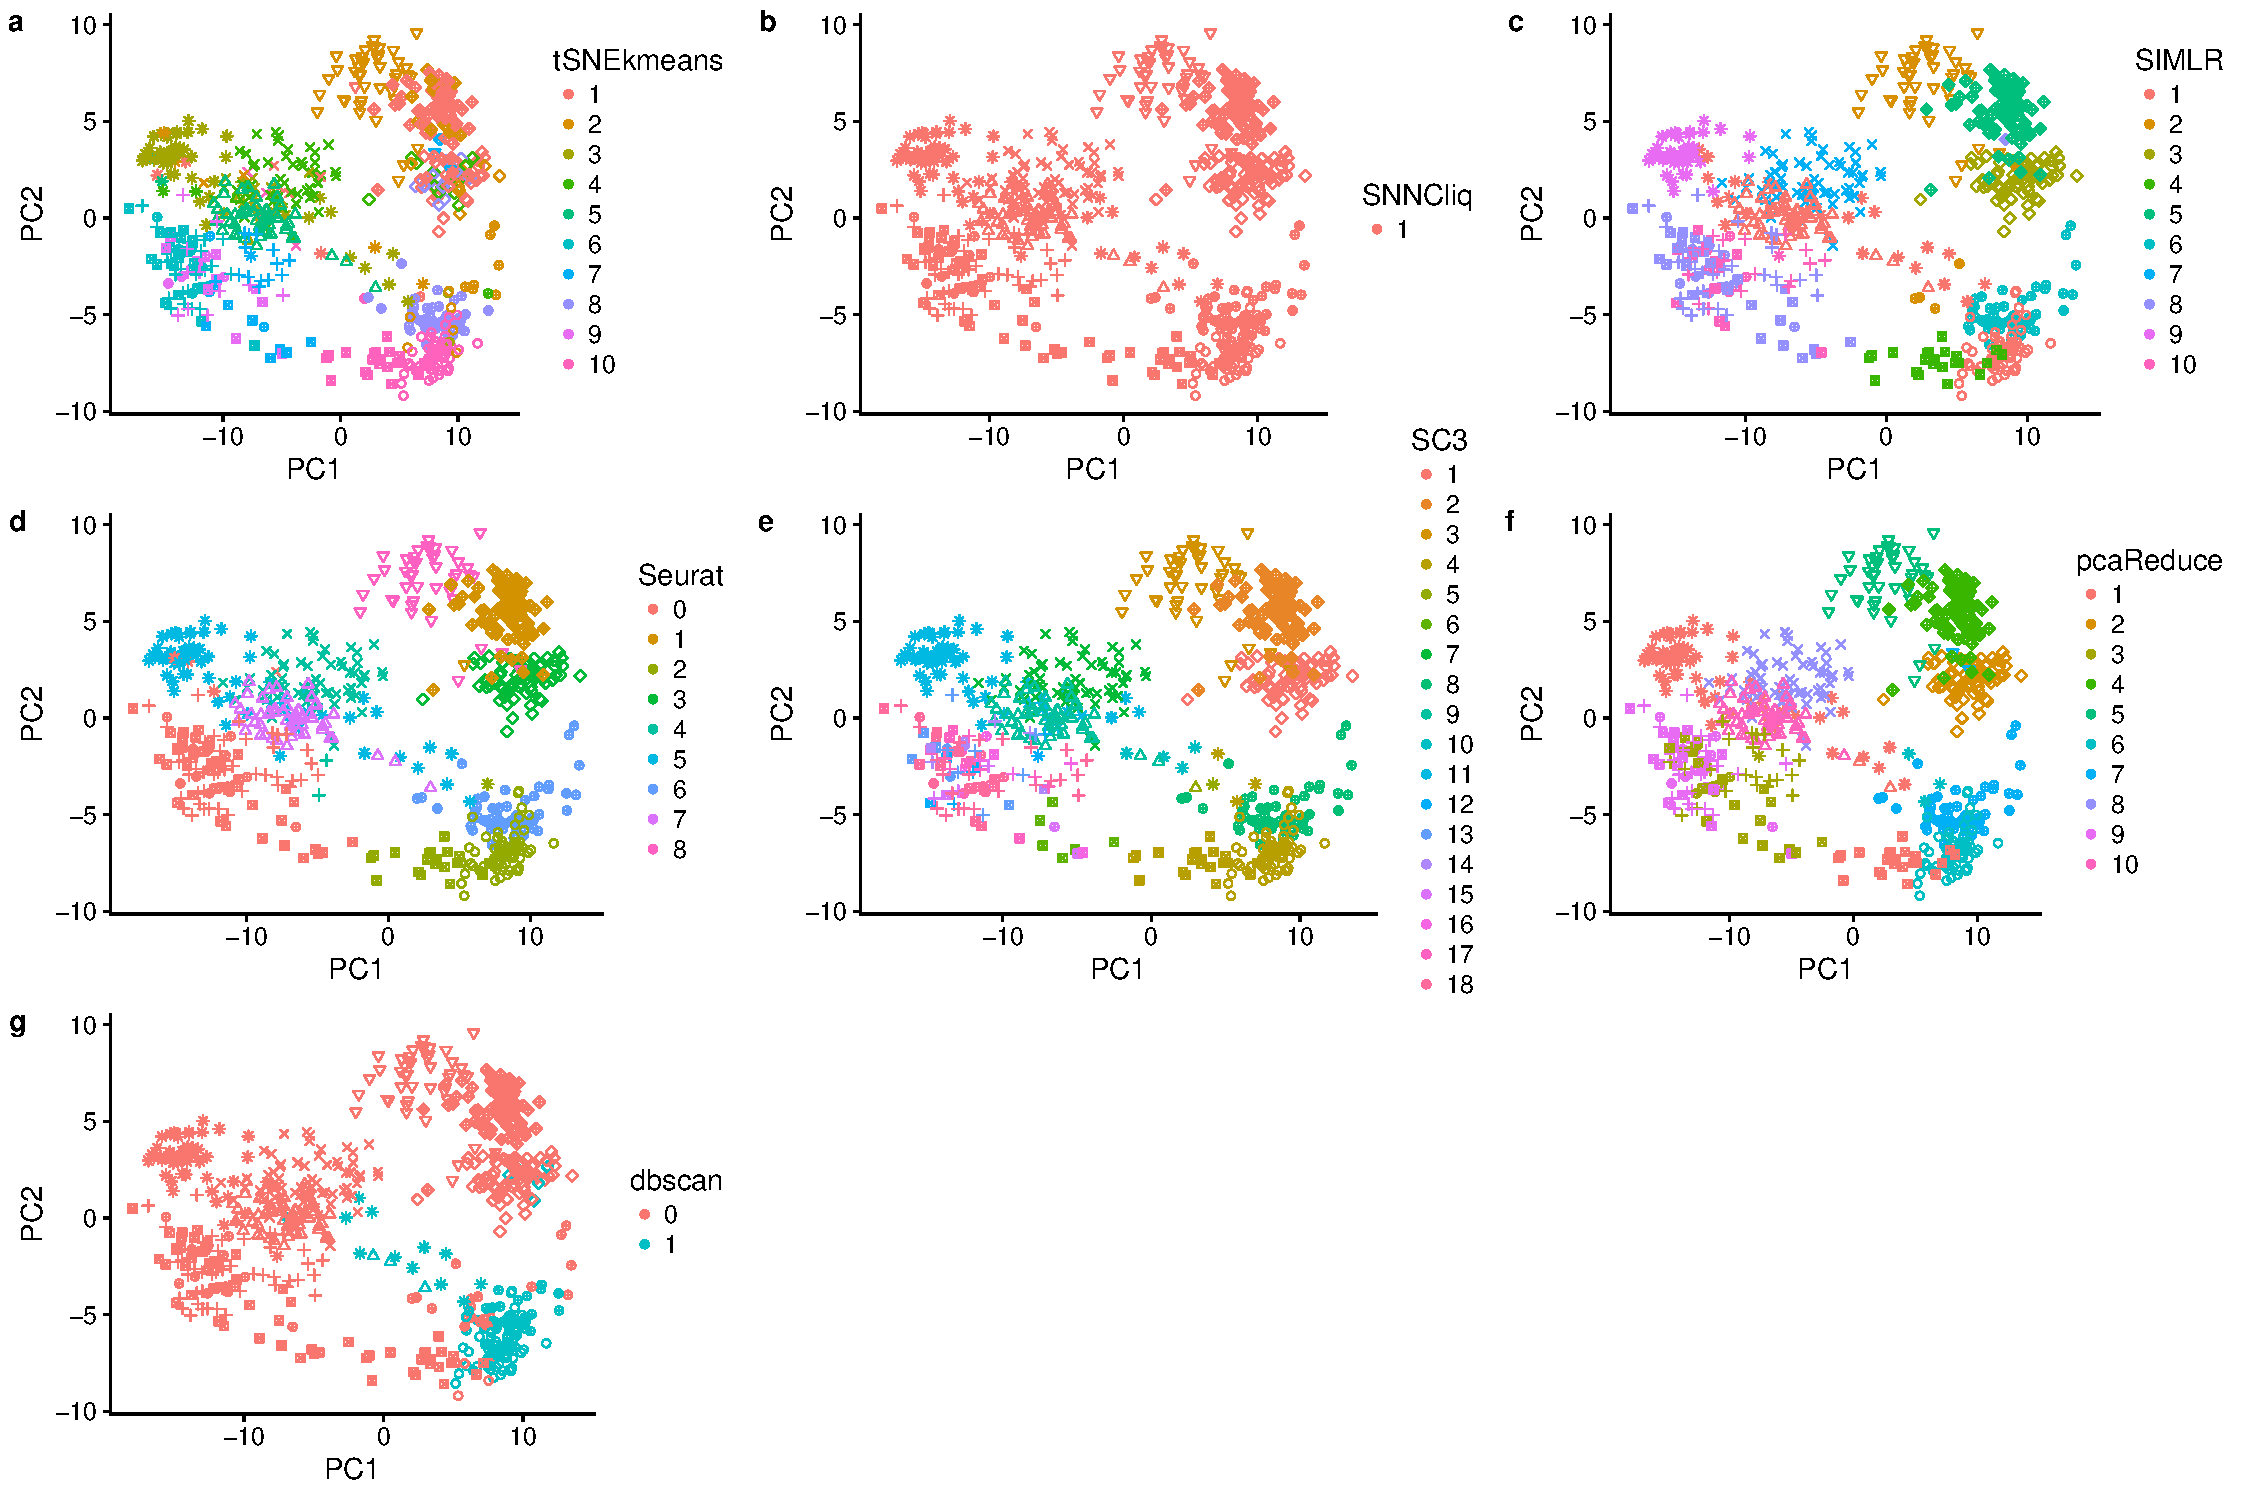
\includegraphics[width=5 in]{/Users/angeloduo/Desktop/masterarbeit/scRNAseq_clustering_comparison/results/plots/plot_cluster_koh2016.pdf}
\caption{Clusters koh2016 on PC representations. }
\label{fig:clusterkoh}
\end{figure}


\begin{figure}[!h]
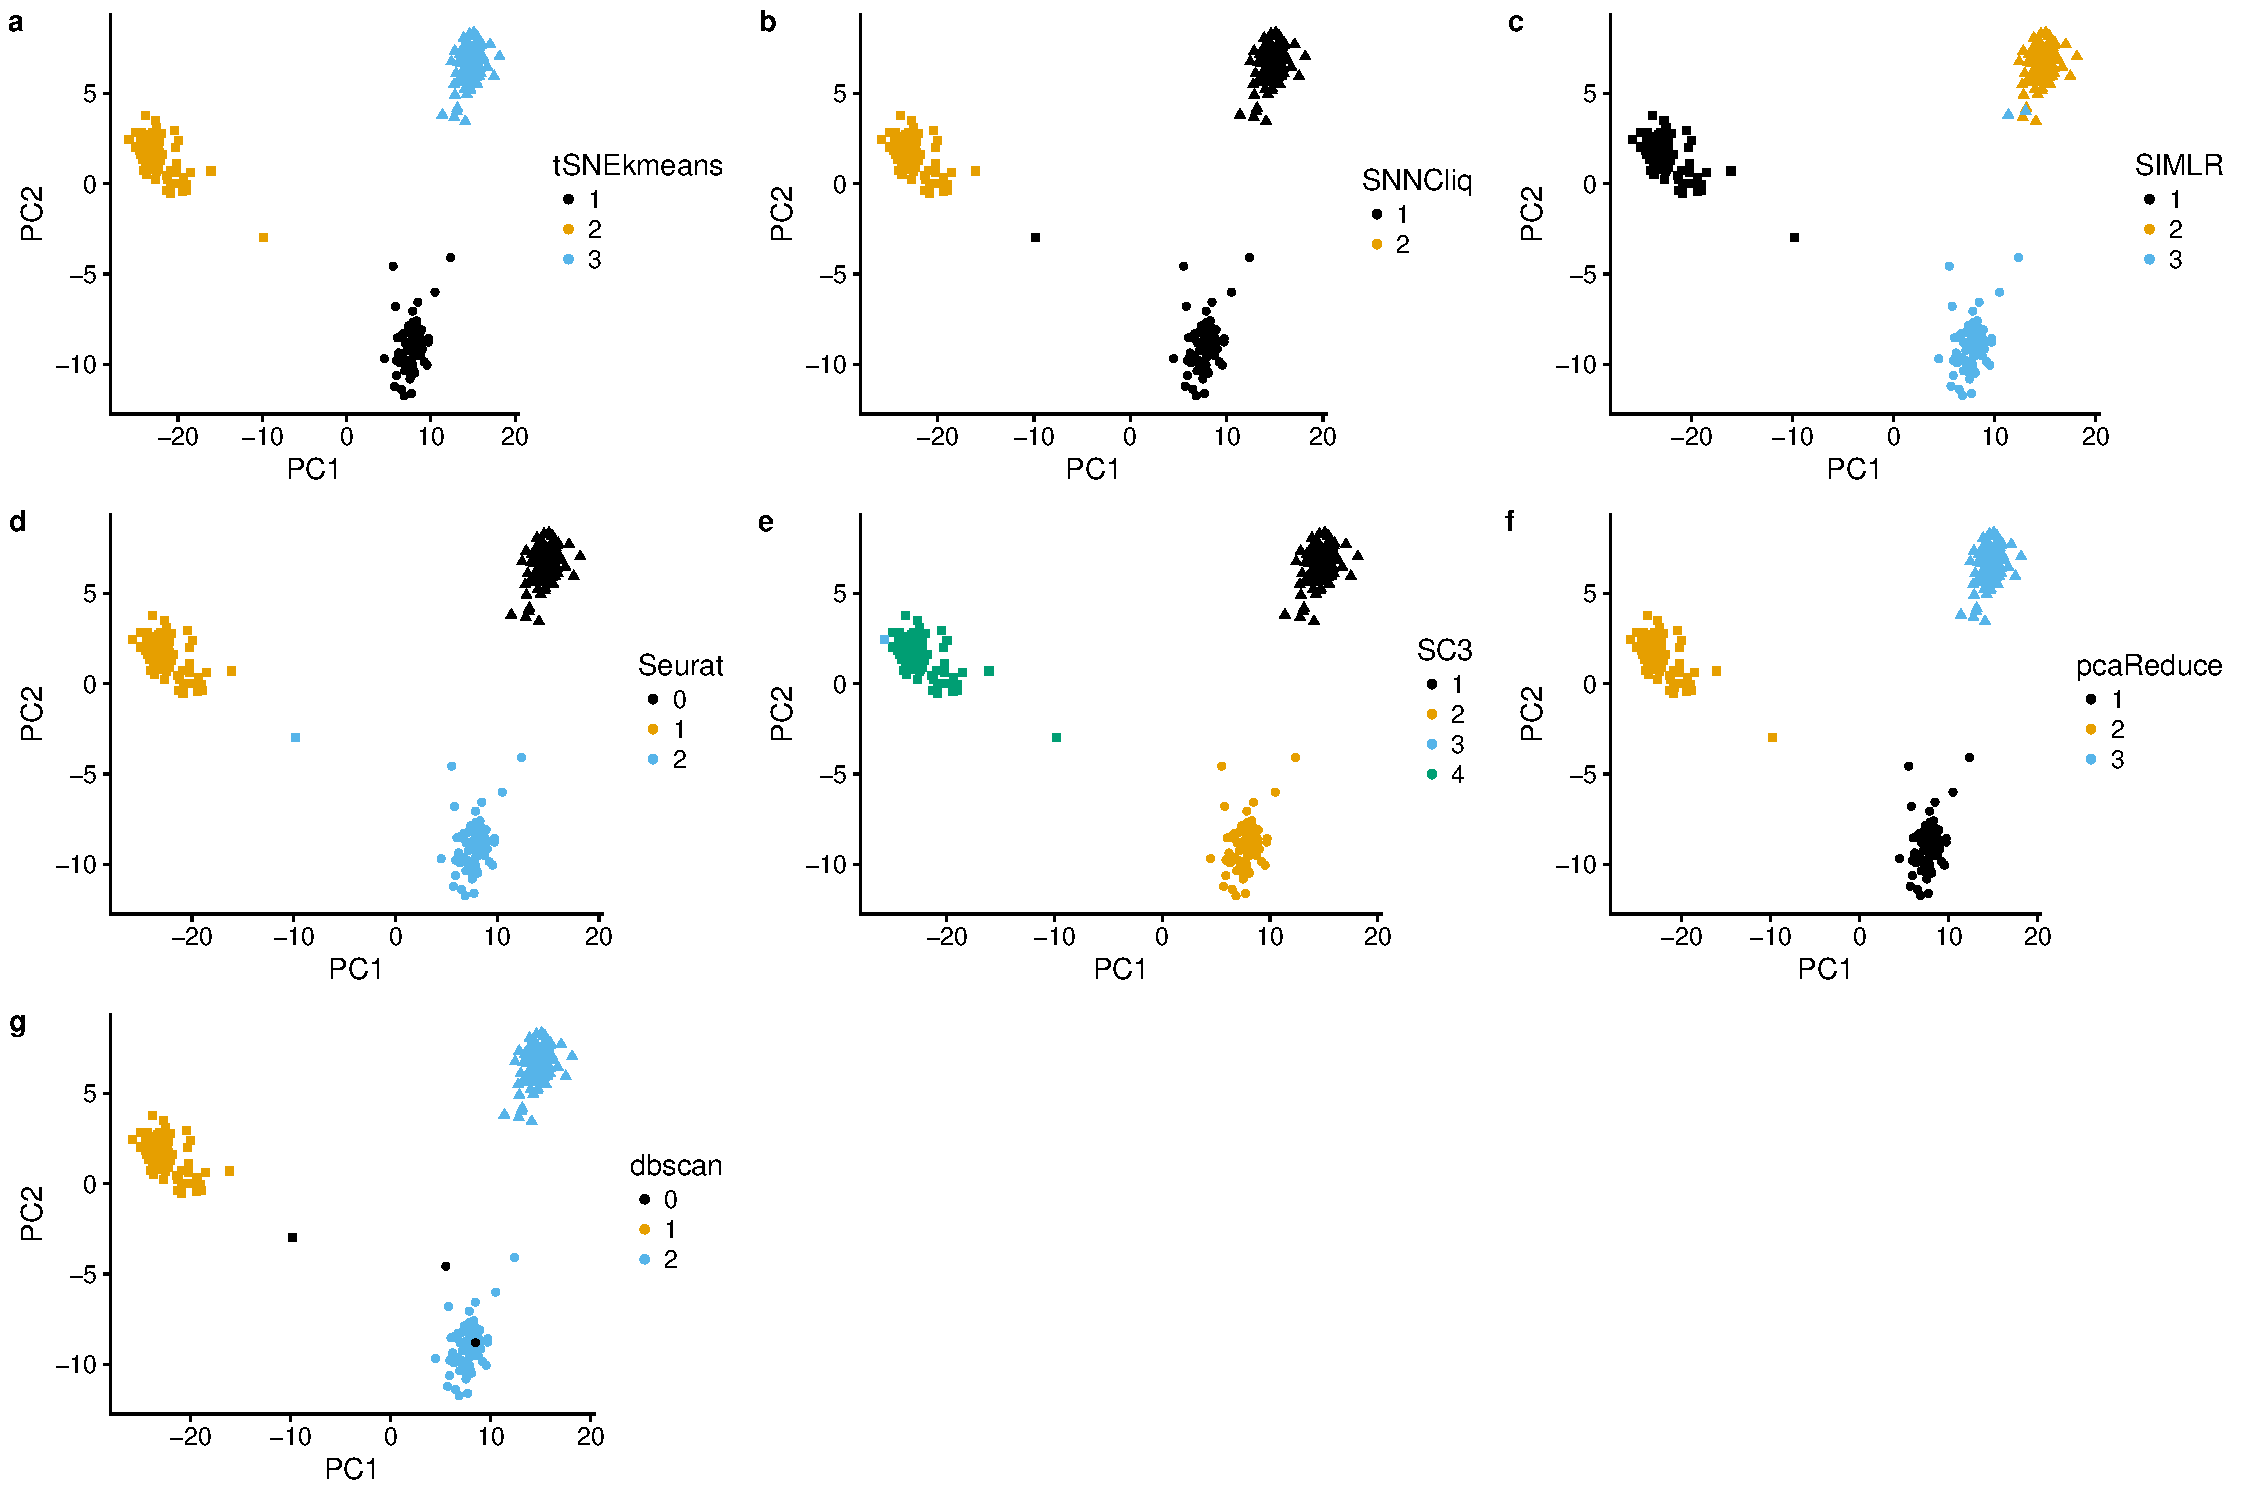
\includegraphics[width=5 in]{/Users/angeloduo/Desktop/masterarbeit/scRNAseq_clustering_comparison/results/plots/plot_cluster_kumar2015.pdf}
\caption{Clusters Kumar 2015 on PC representations. }
\label{fig:clusterkumar}
\end{figure}

\begin{figure}[!h]
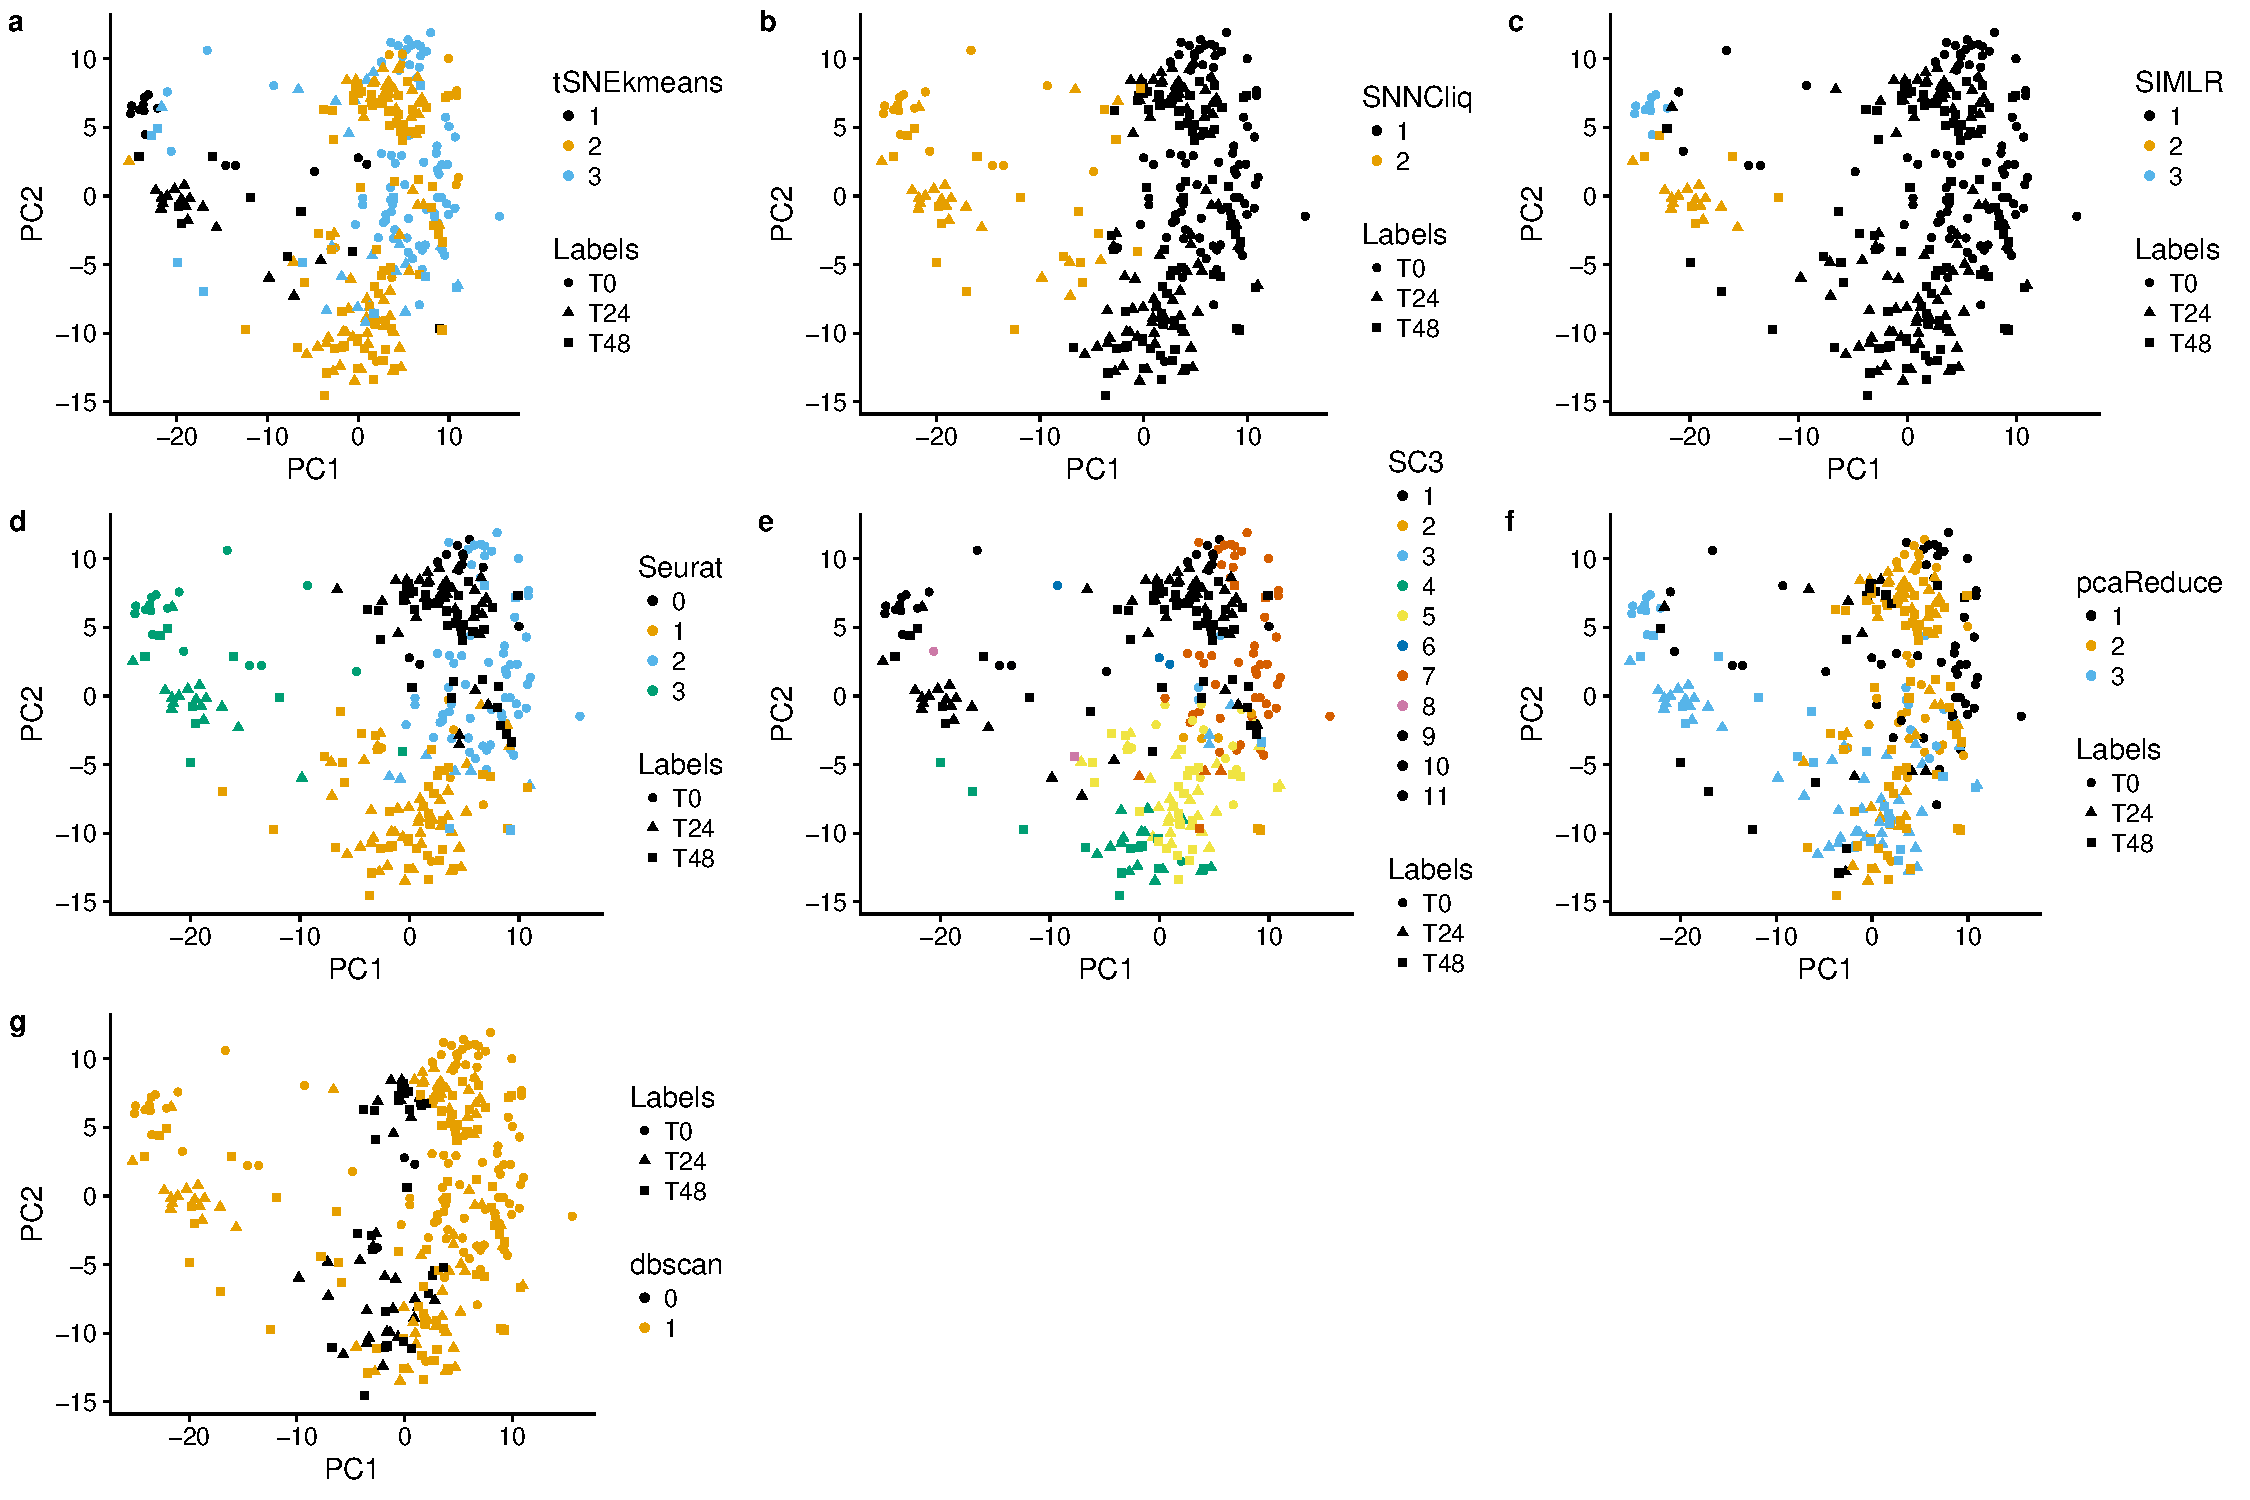
\includegraphics[width=5 in]{/Users/angeloduo/Desktop/masterarbeit/scRNAseq_clustering_comparison/results/plots/plot_cluster_trapnell2014.pdf}
\caption{Clusters Trapnell 2014 on PC representations. }
\label{fig:clustertrapnell}
\end{figure}

\clearpage
\begin{table}[ht]
\centering
\begin{tabular}{rllllll}
  \hline
 & method & parameters & default & annotated k & highest ARI (from k range) & X6 \\ 
  \hline
1 & cidr & n & NULL & NULL &  &  \\ 
  2 & cidr & nCluster & NULL & k &  &  \\ 
  3 & cidr & nPC & 4 & 4 &  &  \\ 
  4 & cidr & cMethod & wardD2 & wardD2 &  &  \\ 
  5 & dbscan & eps & user & user &  &  \\ 
  6 & dbscan & minPts (kNN) & 5 & 0.1 &  &  \\ 
  7 & linnorm & minZeroPortion & 0.75 & 0.75 , (0.25 for Zheng) &  &  \\ 
  8 & linnorm & num\_PC & 3 & 3 &  &  \\ 
  9 & linnorm & num\_Center & 1 to 20 & k &  &  \\ 
  10 & RaceID & min.total & 3000 ( 200 for Zheng) & 3000 ( 200 for Zheng) &  &  \\ 
  11 & RaceID & max.expr & Inf & Inf &  &  \\ 
  12 & RaceID & min.expr & 5 & 5 &  &  \\ 
  13 & RaceID & minnumber & 1 & 1 &  &  \\ 
  14 & RaceID & do.gap & TRUE & FALSE &  &  \\ 
  15 & RaceID & clustrnr & 20 & 0 &  &  \\ 
  16 & RaceID & cln & 0 & k &  &  \\ 
  17 & Rtsnekmeans & k & k & k &  &  \\ 
  18 & Rtsnekmeans & Perplexity & 30 & 30 &  &  \\ 
  19 & Rtsnekmeans & initial\_dims & 50 & 30 &  &  \\ 
  20 & SIMLRlargescale & c & k & k &  &  \\ 
  21 & SIMLRlargescale & k & 10 & 10 &  &  \\ 
  22 & SIMLRlargescale & kk & 100 & 100 &  &  \\ 
  23 & SIMLRlargescale & normalize & FALSE & FALSE &  &  \\ 
  24 & SIMLR & c & k & k &  &  \\ 
  25 & SIMLR & k & 10 & 10 &  &  \\ 
  26 & SIMLR & kk & 100 & 100 &  &  \\ 
  27 & SIMLR & normalize & FALSE & TRUE &  &  \\ 
  28 & SIMLR & no.dim &  &  &  &  \\ 
  29 & tscan & minexpr\_percent & 0.1 to 0.5 & 0.1 to 0.5 &  &  \\ 
  30 & tscan & clusternum & 2 to 20 & k &  &  \\ 
  31 & SC3 & ks & 2 to 10 & elbowplot &  &  \\ 
  32 & SC3 & k\_estimator & TRUE & FALSE &  &  \\ 
  33 & SEURAT & k.param & 30 & 10 percent &  &  \\ 
  34 & SEURAT & dims.use & NULL & screeplot &  &  \\ 
  35 & SEURAT & reduction.type & pca & pca &  &  \\ 
  36 & SEURAT & resolution & 0.8 & 0.8 &  &  \\ 
  37 & pcaReduce & q & 30 & 30 &  &  \\ 
  38 & pcaReduce & nbt & 100 & 100 &  &  \\ 
   \hline
\end{tabular}
\end{table}

% =======================================
% \section{References} \label{sec:ref}
% =======================================
\clearpage

\bibliography{/Users/angeloduo/Desktop/masterarbeit/scRNAseq_clustering_comparison/summary/scRNAseq_clustering.bib}


\end{document}
